% ****** Start of file apssamp.tex ******
%
%   This file is part of the APS files in the REVTeX 4.2 distribution.
%   Version 4.2a of REVTeX, December 2014
%
%   Copyright (c) 2014 The American Physical Society.
%
%   See the REVTeX 4 README file for restrictions and more information.
%
% TeX'ing this file requires that you have AMS-LaTeX 2.0 installed
% as well as the rest of the prerequisites for REVTeX 4.2
%
% See the REVTeX 4 README file
% It also requires running BibTeX. The commands are as follows:
%
%  1)  latex apssamp.tex
%  2)  bibtex apssamp
%  3)  latex apssamp.tex
%  4)  latex apssamp.tex
%
\documentclass[%
 reprint,
%superscriptaddress,
%groupedaddress,
%unsortedaddress,
%runinaddress,
%frontmatterverbose, 
%preprint,
%preprintnumbers,
%nofootinbib,
%nobibnotes,
%bibnotes,
 amsmath,amssymb,
 aps,
%pra,
%prb,
%rmp,
%prstab,
%prstper,
%floatfix,
]{revtex4-2}

\usepackage{graphicx}% Include figure files
\usepackage{dcolumn}% Align table columns on decimal point
\usepackage{bm}% bold math
%\usepackage{hyperref}% add hypertext capabilities
%\usepackage[mathlines]{lineno}% Enable numbering of text and display math
%\linenumbers\relax % Commence numbering lines

%\usepackage[showframe,%Uncomment any one of the following lines to test 
%%scale=0.7, marginratio={1:1, 2:3}, ignoreall,% default settings
%%text={7in,10in},centering,
%%margin=1.5in,
%%total={6.5in,8.75in}, top=1.2in, left=0.9in, includefoot,
%%height=10in,a5paper,hmargin={3cm,0.8in},
%]{geometry}

\begin{document}

\preprint{APS/123-QED}

\title{Distinguishing Anomalous Subdiffusion for Random Walks on Percolation structures and Fractional Brownian Motion}


\author{Ian Jorquera}%
 \email{ian.jorquera@colostate.edu}
\affiliation{%
 Colorado State University, Department of Mathematics
}%


\date{\today}% It is always \today, today,
             %  but any date may be explicitly specified

\begin{abstract}
Random walk statistics can help distinguish between different types of anomalous diffusion. Looking at fractional Brownian motion and random walks on fractal-like structures we compute the mean square displacement, the power spectral density and its coefficient of variance in order to better understand the differences in these types of subdiffusion. We found noticeable differences in the power spectral densities for FBM and random walks on percolation structures at criticality, suggesting such a statistic would be effective in differentiating different types of subdiffusion. The coefficient of variance we saw that both FBM and random walks on percolation structures were relatively indistinguishable,.
\end{abstract}

%\keywords{Suggested keywords}%Use showkeys class option if keyword
                              %display desired
\maketitle

%\tableofcontents

\section{Introduction}
\label{sec:intro} 
In this paper we will look at random walk statistics, such as the power spectral density(PSD) and its coefficient of variation and use these to help determine the structure random walks. In this paper we will restrict our analysis to two different instance of ergodic anomalous subdiffusion: random walks on percolation structures at criticality and fraction Brownian motion (FBM) with $H< \frac{1}{2}$. Anomalous diffusion is when the mean squared displacement of a random walk grows according to a power law over time, that is $\langle r^2(t)\rangle\sim t^\alpha$ for $\alpha\neq 1$, and anomalous subdiffusion is the particular case where $0< \alpha <1$. Ergodicity, is the case where a random walk experiences aging which can be seen when the temporal MSD varies with the total time interval being observed. Anomalous diffusion occurs frequently in biological processes such as in macromolecular crowding, transient binding\cite{krapf_spectral_2019}, diffusion in plasma membranes\cite{weigel_ergodic_2011}, protein configurations, and in modeling the movement of water molecules on the surface of proteins\cite{krapf_strange_2019}.
%Furthermore fractals, and particularly random fractals appear frequently in nature and stocastic process, and our 

However the cause of anomalous behavior can vary greatly, anomalous diffusion can be the result of continuous time random walks (in which case the random walk is non-ergodic), fractional Brownian motion, and random walks on fractal structures\cite{weigel_ergodic_2011, meroz_subdiffusion_2010}. The cases of anomalous diffusion we are interested in are the cases where the anomalous diffusion is the result of the structure of the walk itself (either in the correlation between steps or the landscape in which the walk occurs) and is not related to time intervals between steps. Distinguishing which model best represents the anomalous diffusion is important in determining properties of the underlying diffusion being modeled, and can give insights into the biological processes. The PSD in particular has been shown to be stable on individual trajectories of fractional Brownian motion which is why we are considering this statistic in the context of random walks on fractals\cite{krapf_spectral_2019}. Often data sets may not contain enough data for stable ensemble averages, and so statistics that are stable on individual trajectories are of great interest.

In section \ref{sec:theory} we will look at the theoretical and numerical properties of fractional Brownian motion (FBM), and random walks of percolation structures at, or near, criticality. We will also present the power spectral density and its coefficient of variation. In section \ref{sec:numbers} we will use numerical simulations to simulate both fractional Brownian motion and random walks on percolation structures, in which we will compute the mean squared displacements and the statistics presented in section \ref{sec:theory} to distinguish different types of diffusion.
\section{Theoretical derivations}
\label{sec:theory}
In this section we will present the construction of both fractional Brownian motion and random walks on percolation structures. As well as the definitions for the power spectral density (PSD) and its coefficient of variation, as well as known results for FBM.

\subsection{Fractional Brownian Motion}
Fractional Brownian motion is often used to model movement in crowded or viscoelastic fluids such as the cytoplasm of cells or modeling the movement of polymers\cite{ernst_fractional_2012, CHAKRAVARTI19979}. FBM is determined by its autocorrelation function, where for any $t_1$ and $t_2$, $\langle r(t_1)r(t_2)\rangle=K(t_2^{2H}+t_1^{2H}-|t_2-t_1|^{2H})$, where $0< H< 1$ is the Hurst exponent and $\langle r^2(t)\rangle\sim t^{2H}$. In this paper we will restrict our interest to the case of subdifussion, when $H< \frac{1}{2}$, which correspond to steps being negatively correlated, with an increased likely hood that steps will change direction. Fraction Brownian Motion is the most general Gaussian process and so encapsulated a large number of instances of subdiffusion\cite{krapf_spectral_2019}. A realization of subdiffusive FBM is shown in figure \ref{fig:fbm_r}. The authors of \cite{enriquez_simple_2004} present different approaches for modeling fractional Brownian motion but for this paper we have used the Matlab implementation of the function wfbm for each dimension of our 2 dimensional realizations. Our implementation can be found in the appendix.

\begin{figure}
    \centering
    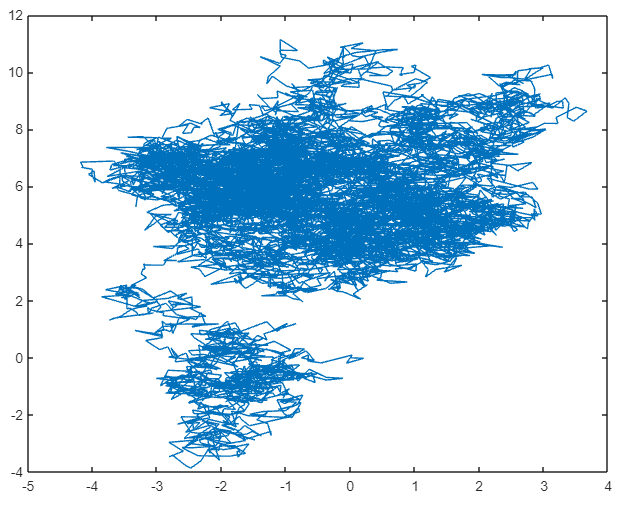
\includegraphics[scale=0.48]{fbm_realization_h35_n10000.png}
    \caption{A realization of $n=10000$ steps of subdiffusive fractional Brownian motion with Hurst exponent $H=.35$}
    \label{fig:fbm_r}
\end{figure}

\subsection{Random Walks on Fractals}
The second case of anomalous subdiffuion we will focus on is the case of a random walk on a fractal. Fractals can occur commonly in nature, sometimes in unexpected ways and so are an important topic of research. The cortical cytoskeleton of kidney cells has been shown to be a scale-free fractal\cite{krapf_strange_2019}. Fractal structures are also found in epidemiology and in tracking forest fires to model aspects of spread \cite{buldyrev_fractals_2009} and in modeling walks on infinite (or pseudo-infinite) graphs\cite{masuda_random_2017}. Generally random walks on fractals are done by first generating a fractal (a common example is the Serpinski Gasket) or a fractal-like lattice (such as a percolation structure) and then having a random walker jump randomly along the available sites\cite{ben-avraham_diffusion_2000, dauriac_random_1983}. To simulate our random fractals we will create percolation structures at critically. A percolation structure is a multidimensional grid where each cell, or site, can either exist with probability $p$ or not. This means we can generate a percolation structure by generating a multi-dimensional binary array where each site exists with probability $p$. For our purposes we will look at percolation structures at critically meaning $p=p_c$ the probability of criticality, at which point an infinite cluster exists and the percolation structure shares the properties of a random fractal\cite{ben-avraham_diffusion_2000}.

A random walk on a fractal will walk along the percolation structure by jumping between adjacent existing sites. This means the possible directions a walker can take will vary depending on where the walker is on the percolation structure. This also leads to backtracking where the walker has to retrace its self at each dead end along the walk. On a 2 dimension grid where a walker can move in any of the 4 direction: up, down, left, right it is know that $p_c\approx 0.59275$, an infite cluster on such a percolation structure is shown in figure \ref{fig:perc}. In our analysis we will focus on percolation structures of this type. It also know that the fractal dimension of such a percolation structure is $d_f=1.896$ and the dimension of any walk on this percolation structure is $d_w\approx 2.878$, meaning we expect to see the MSD to be $\langle r^2(t)\rangle\sim t^{\alpha}$ where $\alpha\approx 0.69$\cite{ben-avraham_diffusion_2000}.

\begin{figure}
    \centering
    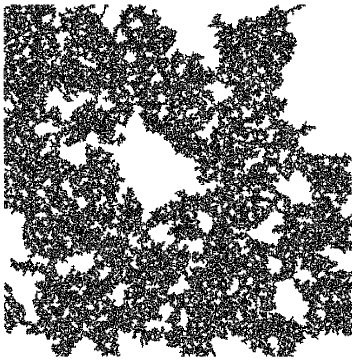
\includegraphics[scale=.6]{perc_infcluster.PNG}
    \caption{An infinite cluster in a percolation on a square lattice with $p\approx p_c$, from \cite{ben-avraham_diffusion_2000}. Sites not on the infinite cluster have been removed for clarity}
    \label{fig:perc}
\end{figure}

\subsection{The Power Spectral Density}
For a realization, or a random trajectory of length $T$, we can write the trajectory a as sequence of steps $(\textbf{R}_t)_t$, which represent a realization of a random walk over the time interval from $0$ to $T$, where for each step $\textbf{R}_t=(X_t^{(1)}, X_t^{(2)},\dots, X_t^{(d)})$ and the component $X_t^{(i)}$ represent the length of the step in the $i$-dimension. The components of the walk in each dimension can be thought of as a statistically independent $1$-dimensional walks and so we will focus our analysis on the PSD in one fixed dimension. The PSD over an arbitrary fixed dimension $j$ is then defined as the Fourier transform in equation \ref{eq:psd_traj}\cite{krapf_spectral_2019}.

\begin{equation}
\label{eq:psd_traj}
    S(f,T)=\frac{1}{T}\left|\int_{0}^T \text{exp}(ift)X^{(j)}_t \, dt\right|^2
\end{equation}

The general PSD over all dimensions is the the sum over all dimensions $j$, but from the statistical independence of each dimension this would be proportional to the PSD in a single dimension. Equation \ref{eq:psd_traj} gives us the PSD for a single trajectory, which we can extend to an ensemble average over multiple runs, which we will denote as $\langle S(f,T)\rangle$.

It is known that the ensemble PSD for subdiffusive fractional Brownian motion (where $H< \frac{1}{2})$ follows a power law $\langle S(f,T)\rangle\sim 1/f^\beta$ where $\beta={2H+1}$\cite{krapf_spectral_2019}.

The PSD is a widely used tool in engineering fields for determining the roughness of surfaces\cite{andren_power_2006, elson_calculation_1995}. This idea can provide a useful intuition behind the meaning of the PSD in the context of random walk, and suggest the PSD encapsulates some fundamental structure of the random walk. The PSD is also used in a variety of other applications such as tracking the fluctuations of current in electrodes\cite{krapf_nonergodicity_2012}, and studying the intervals between earthquakes\cite{sornette_self-organized_1989}.

\subsection{The Coefficient of Variance of the Power Spectral Density}
The final statistic we will present is the coefficient of variance of the PSD. In the previous section we presented the ensemble average, or mean, of the power spectral density, denoted as $\langle S(f,T)\rangle$. In a similar vein we can also talk about the variance and standard deviation of the PSD over many realizations. And so $\sigma^2=\langle S(f,T)^2 \rangle$. We can then define the coefficient of variance of the PSD as shown in equation \ref{eq:coef_var}.

\begin{equation}
\label{eq:coef_var}
    \gamma = \frac{\sigma}{\mu}=\frac{\sqrt{\langle S(f,T)^2 \rangle}}{\langle S(f,T) \rangle}
\end{equation}

In the case of subdiffusive fractional Brownian motion (where $H<\frac{1}{2}$), the coefficient of variance $\gamma\rightarrow 1$ when $\omega=fT\rightarrow \infty$. This is true for an FBM process with $H< \frac{1}{2}$. The coefficient of variance is different for when $H=\frac{1}{2}$ and when $H>\frac{1}{2}$\cite{krapf_spectral_2019}.

\section{Numerical Simulations and Results}
\label{sec:numbers}
In this section we will compute, numerically, the ensemble MSD, PSD and the coefficient of variance for random walks on fractals and fraction Brownian motion and compare the results with the theoretical expectations of FBM.

First we will simulate random walks on fractals, using percolation structures. An example realization is shown in figure \ref{fig:perc_real}. We then computed $7000$ realizations of random walks with $4500$ steps. We then computed the ensemble MSD to be $\langle r^2(t)\rangle\sim t^{0.707}$ (as compared to the predicted value of $\alpha=0.69$), which is shown in figure \ref{fig:linmsd_frac}. This corresponds to the fractal dimension of the walk being $d_w=2.83$ (as compared to the theoretical value of $2.878$). It is important to note that we considered only the realizations on the infinite cluster, this means we excluded any realization that visited too few distinct sites. See Appendix for the implementation on how we achieved this.

\begin{figure}
    \centering
    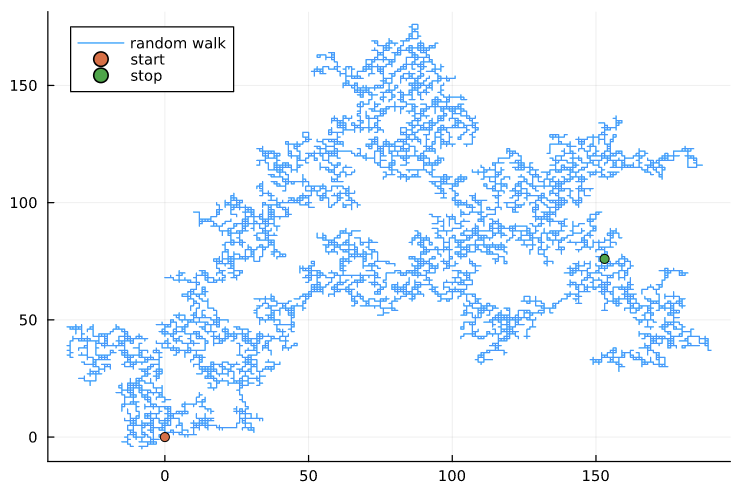
\includegraphics[scale=.49]{frac_realization_n10000.png}
    \caption{A realization of $n=45000$ steps of a random walk on a percolation with $p\approx p_c$}
    \label{fig:perc_real}
\end{figure}

\begin{figure}
    \centering
    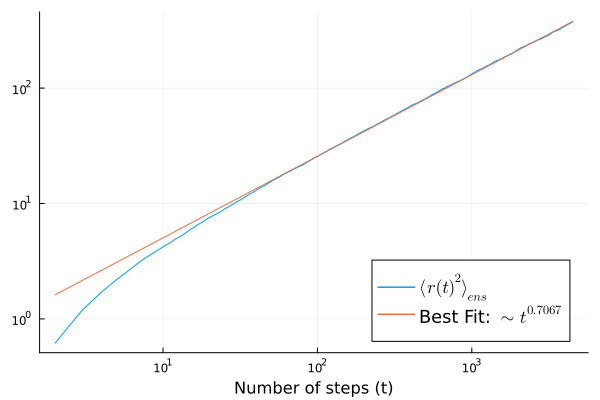
\includegraphics[scale=.36]{lin_ens_msd_frac.png}
    \caption{A $\log$-$\log$ linearization of the ensemble MSD for random walks on fractals}
    \label{fig:linmsd_frac}
\end{figure}

To compare random walks on percolation structures to FBM, we then generated $5000$ realizations of FBM with Hurst exponent $H=.35$ which will correspond to a theoretical MSD that grows at roughly the same rate as the fractal walk. We verified the ensemble MSD of these realizations and found $\langle r^2(t)\rangle\sim t^{0.709}$, which matched the theoretical predictions and the the random walks on percolations structures. A linearized MSD for FBM is show in figure \ref{fig:linmsd_fbm}.

\begin{figure}
    \centering
    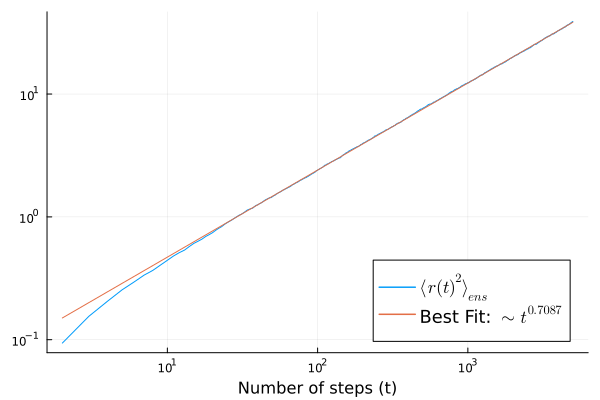
\includegraphics[scale=.36]{lin_ens_msd_fbm.png}
    \caption{A $\log$-$\log$ linearization of the ensemble MSD for fractional Brownian motion}
    \label{fig:linmsd_fbm}
\end{figure}

At this point both ensemble MSDs seem to correspond to similar instances of anomalous sub diffusion as both share the same power law for their MSDs. However both instances were generated using vastly different methods. We then compared the two statistics presented in section \ref{sec:theory}. First we computed the PSD for each set of instances. First for fractional Brownian motion we found that the ensemble PSD (shown in figure \ref{fig:lin_psd_fbm}) grows as the power law $\langle S(f,T) \rangle\sim 1/f^{1.703}$, which aligns with the theoretical prediction of $\beta=1.7$.

\begin{figure}
    \centering
    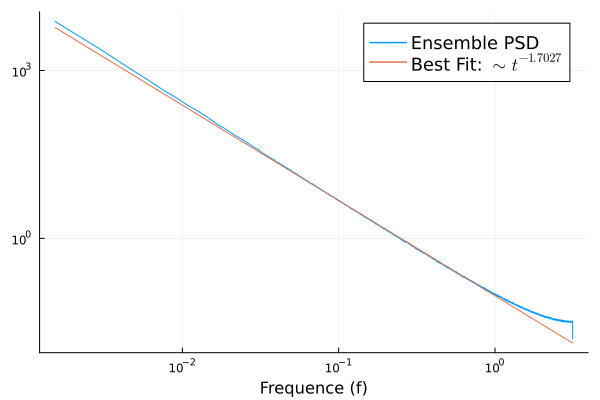
\includegraphics[scale=.36]{lin_ens_psd_fbm.png}
    \caption{A $\log$-$\log$ linearization of the ensemble PSD for fractional Brownian motion}
    \label{fig:lin_psd_fbm}
\end{figure}

We then computed the ensemble PSD for the random walks on percolation structures at criticality. We found that the ensemble PSD (shown in figure \ref{fig:lin_psd_frac}) grows as the power law $\langle S(f,T) \rangle\sim 1/f^{1.802}$. Notice that the power laws for FBM and random walks on fractals differ which indicated that the PSD and power law growth is in fact an effective way to distinguish between FBM and random walks on fractals. This also suggest that these two instances of sub-diffusion have different in there structure even though they have similar MSDs.

\begin{figure}
    \centering
    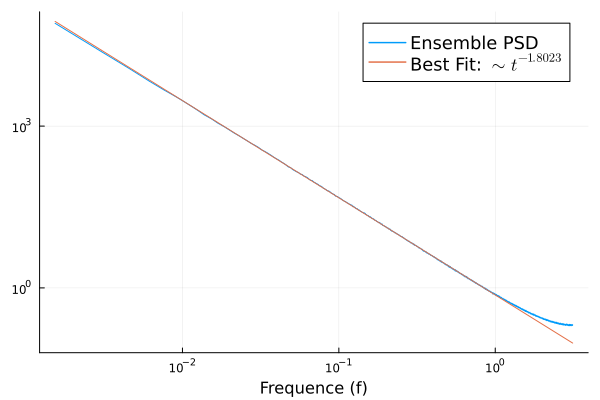
\includegraphics[scale=.36]{lin_ens_psd_frac.png}
    \caption{A $\log$-$\log$ linearization of the ensemble PSD for random walks on fractals}
    \label{fig:lin_psd_frac}
\end{figure}

Next we will look at the coefficient of variance, which is computed according to equation \ref{eq:coef_var} where we look at the limiting behavior for large $\omega=fT$. For fractional Brownian motion we computed $\gamma\approx 1.0045$ which aligns with the theoretical prediction of $1$. Similarly for the random walks on the percolation structures we computed $\gamma\approx 1.0174$ which seems to be indistinguishable from the coefficient of variance for FBM. This indicates that the coefficient of variance does not accurately distinguish between FBM and random walks of fractals. This result, with the known theoretical result of fraction Brownian motion, also suggest that the coefficient of variance may be common result amongst all instances of anomalous subdiffusion, that of a coefficient of variance equal to $1$. However more types of subdiffusion need to be considered for such a conclusion.

Percolation structures are easy to generate but do not represent a wide variaty of fractal like stuctures. Percolation structures only share the properties of fractals when the probability $p$ of a site existing is near criticality $p_c$. Otherwise random walks on percolation structures may act more similar to those on finite graphs or that of normal diffusion. This limitation of the variability of percolation structures acts as a major limitation to our results. Further research can be done looking at a variety of different percolation structures, and on well defined fractals.

\section{Conclusion}
In this paper we looked at the random walk statistics of power spectral density and the coefficient of variance to determine how either statistic could be used to distinguish between different instances of anomalous subdiffusion. We looked at fractional Brownian motion and random walks on fractal like structures. We found that there was likely a noticeable difference between the power law growth of FBM and random walks on a percolation structures at criticality, indicating that the PSD would be a good statistic for distinguishing between different types of subdiffusion. This also suggests random walks on fractals have a different fundamental structure then random walks with fractional Brownian motion. For the coefficient of variance we saw that both FBM and random walks on percolation structures were relatively indistinguishable. This suggest the coefficient of variance may be a common statistic for many types of subdiffusion, with different structure, but can not be used to distinguish them.

\appendix

\section{Simulations}

Code for this project can be found our the github \href{https://github.com/jorqueraian/walking-randomly}{https://github.com/jorqueraian/walking-randomly}

%To start 
% The \nocite command causes all entries in a bibliography to be printed out
% whether or not they are actually referenced in the text. This is appropriate
% for the sample file to show the different styles of references, but authors
% most likely will not want to use it.

\bibliography{apssamp}% Produces the bibliography via BibTeX.

\end{document}
%
% ****** End of file apssamp.tex ******
